\documentclass[letterpaper,12pt]{article}
\usepackage[parfill]{parskip} % Remove paragraph indentation
\usepackage{amsmath}
\usepackage{float}
\usepackage[margin=1in]{geometry}
\usepackage{graphicx}
\usepackage{placeins}
\usepackage{siunitx}
\usepackage[title]{appendix}
\usepackage{pdflscape}
\usepackage{tabularx}
\usepackage{times}
\usepackage{url}
\usepackage{setspace}
\usepackage[none]{hyphenat}
\usepackage{pdfpages}
\usepackage{longtable}

\DeclareSIUnit{\samplepersec}{SPS}

\begin{document}

\begin{titlepage}
    \begin{center}
        \vspace*{1cm}

        \Large
        \textbf{ELEC 490/498 Project Blueprint Document}

        \vspace{0.5cm}
        Group 18\\
        TeachEE\\
        \vspace{0.5cm}
        \normalsize
        \textbf{John Giorshev (20103586, john.giorshev@queensu.ca) \\ Eric Yang (20120750, e.yang@queensu.ca) \\ Ethan Peterson (20105011, 17emp5@queensu.ca) \\ Timothy Morland (20096286, 17tm22@queensu.ca)}\\
        \vspace{0.5cm}
        Submitted November 22, 2022\\

        \vfill
            
        \textbf{To:}\\
        Instructor and Supervisor Dr. Sean Whitehall (sw109@queensu.ca) \\
        Supervisor Dr. Thomas Dean (tom.dean@queensu.ca) \\
            
        \vspace{1.8cm}

    \end{center}
\end{titlepage}
\section{Executive Summary}

This report outlines TeachEE, a device which facilitates online learning for
electrical engineering labs. It describes the project's scope: a minimum viable
product for the purpose of this capstone project, with room for scope expansion
later in the year if circumstances allow it. The minimum viable product consists
of an oscilloscope, desktop app, and communication between a computer and the
device via USB. A complete list of specifications for the MVP are provided in
Table \ref{hw:specs-table} and Table \ref{sw:specs-table}.

It also outlines a road-map for this project; most hardware related tasks have
been completed, with the software related tasks scheduled for completion later
in the term. Although the PCB shipment from the manufacturer was delayed, the
project is still on schedule. Additionally, for the upcoming tasks, there is a
clear and equal division of responsibility between group members, as shown in
Table \ref{hw:milestones-table}. The project is scheduled to be completed by
week 20, two weeks before the Open House, to allow for extra time in case of
emergencies.

\tableofcontents
\listoffigures
\listoftables
\newpage
\setstretch{1.5}
\section{Introduction} \label{sec:intro} % Ethan
This blueprint outlines Group 18's capstone project TeachEE, which was
originally proposed in ELEC390 \cite{prop_390}. This report is intended for the
ELEC 498 instructors and Group 18's supervisors. The report provides the
baseline specifications for TeachEE. These specifications should be treated as
the minimum performance required for the showcase of the project in March. This
blueprint consists of the methodology of completing the project, progress up to
the time of writing this document, budget, and strategies to mitigate issues.
The appendices of this report include technical information that supplements the
report body.

% NOTE: what I had before: (came after remote delivered eng labs)
% At a design level, the device will require
% both a custom Printed Circuit Board, device driver, and graphical user interface
% to function correctly. There are two key technical challenges in this project;
% the Printed Circuit Board (PCB) and device driver software.
\subsection{Design Problem}
TeachEE is a device that acts as a general purpose electronics measurement
instrument for remotely delivered engineering labs. The device acts as both a
USB oscilloscope and current monitor. Currently, there are few instrumentation
options for students completing their labs remotely. The TeachEE bundles
together the functionality most commonly required for electrical engineering
labs and packages it with portable software that can run on lower end computers
with any operating system.
\\~\\
The PCB is a large technical undertaking as the PCB must be able to capture both
voltage and current samples at a rate that is useful to undergraduate student.
Moreover, the PCB must contain custom circuitry to relay the sample data over
USB. USB is a high speed interface requiring controlled impedance transmission
lines on the PCB. Additionally, the PCB will need multiple high speed clocks for
the USB PHY and Analog to Digital Converter (ADC). There are also further
technical challenges with respect to the analog signalling and sufficiently
filtering and protecting the inputs.
\\~\\
The second key technical challenge in this project is the device driver for the
oscilloscope. The USB 2.0 link between the device and laptop has a throughput as
high as 480 Mbps. This requires performant driver software that can process the
sample data in a timely manner and relay it to the GUI frontend. In addition to
the requirement for low latency, the software will also require a packet framing
technique that can efficiently separate current and voltage samples. In regard
to changes from the ELEC390 proposal, our team has removed the voltage power
sources and changed the microcontroller to an FPGA.
% Ethan
% Explain the design problem Hardware software timeline
% 275 words max
\subsection{System Specifications}
Since the TeachEE has both a hardware and software component. The system
specifications have been broken up into hardware and software tables
respectively.

% \newcolumntype{b}{X}
% \newcolumntype{s}{>{\hsize=.2\hsize}X}
% \newcolumntype{m}{>{\hsize=.4\hsize}X}
\begin{table}[h!]
    \caption{Hardware Specifications}
    \begin{tabularx}{\textwidth}{l|l|l|l}
          & Specification & Target Value & Tolerance \\
        \hline
        1 &Voltage Input Bandwidth&\SI{100}{\kilo\hertz}& $\pm \SI{1}{\kilo\hertz}$ \\
        2 &Current Input Bandwidth&\SI{100}{\kilo\hertz}& $\pm \SI{1}{\kilo\hertz}$ \\
        3 &Measureable Current Range&\SI{-15}{\ampere} to \SI{+15}{\ampere}& $\pm \SI{5}{\ampere}$ \\
        4 &Measureable Voltage Range&\SI{0}{\volt} to \SI{3.3}{\volt}& $\pm \SI{200}{\milli\volt}$ \\
        5 &Number of Current Input Channels& $1$ & $0$ \\ 
        6 &Number of Voltage Input Channels& $1$ & $+2$ \\
        7 &Power Input Voltage Rating& \SI{5}{\volt} & $\pm \SI{500}{\milli\volt}$ \\
        8 &Power Current Consumption Rating& \SI{500}{\milli\ampere} & $\pm \SI{250}{\milli\ampere}$ \\
        9 &Voltage Sample Rate& \SI{1}{\mega\samplepersec} & \SI{0}{\mega\samplepersec}\\
        10 &Current Sample Rate& \SI{1}{\mega\samplepersec} & \SI{0}{\mega\samplepersec} \\
        11 &PCB Thickness& \SI{1.6}{\milli\metre} & $\pm \SI{0.1}{\milli\metre}$ \\
        12 &PCB Dimensions& \SI{0.04}{\meter\squared} & $\pm \SI{400}{\milli\metre\squared}$ \\
        13 &Voltage Sample Error against commercial scope & N/A & $\pm \SI{10}{\percent}$ \\
        14 &Current Sample Error against commercial meter& N/A & $\pm \SI{10}{\percent}$
    \end{tabularx} 
\label{hw:specs-table}
\end{table}

% Timbo / Ethan
\begin{table}[h!]
    \caption{Software Specifications}
    \begin{tabularx}{\textwidth}{l|l}
        \textbf{1} & \textbf{Functional Requirements}\\
        \hline
        1.1 & The software shall be able to modulate the sample rate. \\
        1.2 & The software shall be able to modify the trigger voltage. \\
        \hline
        \textbf{2} & \textbf{Interface Requirements} \\
        \hline
        2.1 & Something about driver interface to GUI Idk (write in the formal format I showed above plz) \\
        2.1 & Also try to write some stuff about how FTDI driver interfaces with backend which in turn interfaces with frontend. What are the interface signatures and tools used? \\
        \hline
        \textbf{3} & \textbf{Performance Requirements} \\
        \hline
        3.1 & The software shall be able to render waveforms at a rate of \SI{30}{\hertz} on screen.
    \end{tabularx} 
\label{sw:specs-table}
\end{table}

% 1-2 tables (maybe one for HW SW)
% Ethan will write some hardware and software specs here in a table

\section{Methodology} % ERIC
% 1.5 pages max for everything

\subsection{Approach}

% Software
The software portion of the USB oscilloscope will be a desktop application
displaying the user interface with web technologies. The issue of cost is
addressed here as the display and processing power of the user's machine
can be used in place of additional display and processing hardware. Exporting
sample data to a CSV file will easily be done through a button on the user's
screen. The application will be built using Tauri, a framework that utilizes
a Rust binary as a backend and JavaScript, HTML, and CSS as the frontend.
\\~\\
% Hardware
The TeachEE hardware design will be a standalone PCB which provides an FPGA with
access to USB controller and Analog to Digital Converter (ADC). The FPGA will
not be soldered directly to the PCB, instead the TeachEE will have a socket to
connect an off-the-shelf FPGA module. FPGAs are highly complex with requirements
for multiple clocks and voltage rails. The module will save the team time and
allow the FPGA to be replaced in the event of a hardware failure. A full
hardware system block diagram is given in Figure \ref{fig:pcb-block-diagram}.

\subsection{Design Tools, Hardware, Instrumentation}
Tauri was chosen as the application framework because of its high performance
and low binary size when compared to other Rust frameworks 
\cite{tauri_benchmarks}. As TeachEE is intended for remote use, being
lightweight is important for quick deployment and operation. Tauri also compiles
to all Windows, macOS, and Linux platforms, which allows use of the product no
matter what machine a user may have.
\\~\\
The Rust programming language will be used to address the high throughput and
data processing requirements due to its high run time speed \cite{rust_speed}.
Furthermore, Rust provides support for concurrent programming by preventing race
conditions at compile time. Concurrency may be necessary to speed up data stream
processing (e.g. Fast Fourier Transform).
\\~\\
The frontend will be written in plain JavaScript to avoid the performance
overhead due to abstractions in JavaScript frameworks \cite{javascript_speed}.
Although modularization can improve code maintainability, it is not necessary
for this project because the user interface is intended to be simple.
\\~\\
The primary design tool used for the hardware is Altium with the PDN Analyzer
extension. Altium is full PCB schematic and layout design suite. The software
will also produce fabrication files in a standard format that can be given to
manufacturers. PDN Analyzer provides tools for checking the Power Distribution
Network (PDN) of the PCB. The tool is used as a final verification that the PCB
traces can carry enough current to supply all devices on the board.

\subsection{Validation}
Tauri provides Tauri Action, which is a Github Action that builds Tauri
applications into native binaries on Windows, macOS, and Linux
\cite{tauri_actions}. This feature will be used to provide continuous integration
to the project and ensure correctness on all targeted platforms.
\\~\\
A waveform generator can be used as a test dummy to generate a waveform that
can be compared with the output displayed by measuring it with TeachEE.
This output can also be compared with measurements obtained from a commercial
oscilloscope. Test success will be indicated by voltage/current differences
given by the target percentages in the hardware specifications.

\section{Progress to Date} % Ethan / Tim for HW/SW respectively
Since the start of the term, the team has completed a set of both hardware
software tasks.
% Explain that there has been a completed hardware design.
% include schematics, layout and BOM in Appendices

\subsection{Hardware Design}
As of this blueprint submission, the initial printed circuit board schematic and
layout are complete. The PCB system block diagram is shown in the figure below.
Full schematic and layout prints are supplied in Appendix
\ref{appendix:schematic} and \ref{appendix:layout} respectively.
\begin{figure}[H]
    \centering
    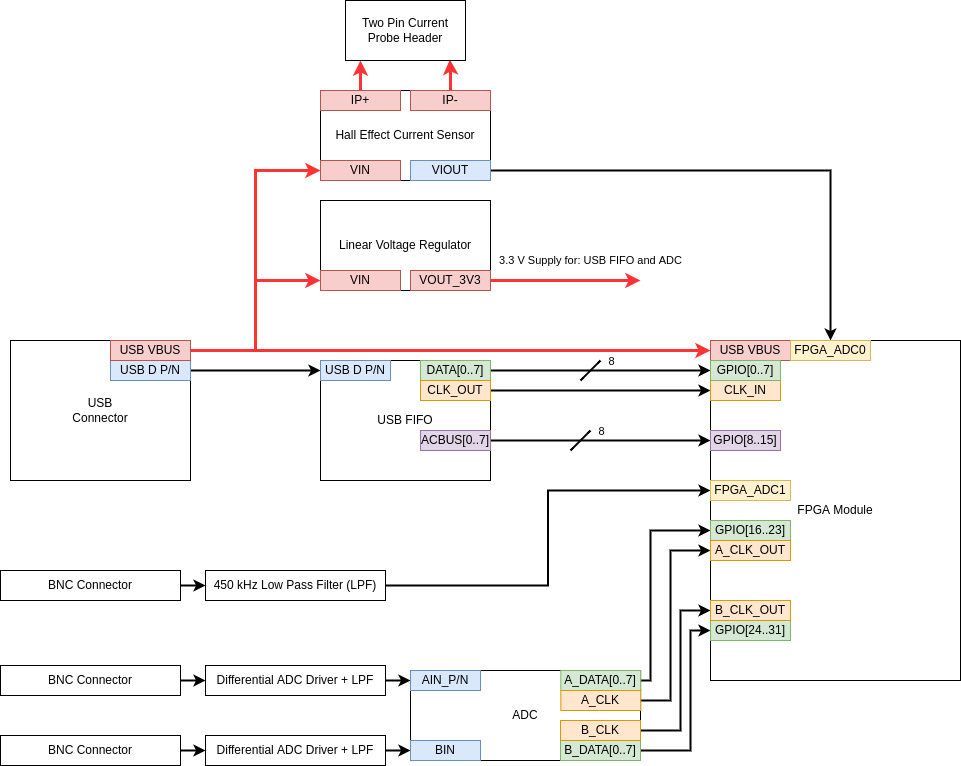
\includegraphics[width=16cm]{../../misc/TeachEE-System-Diagram.drawio.png}
    \caption{TeachEE PCB System Block Diagram}
    \label{fig:pcb-block-diagram}
\end{figure}

The block diagram above is a simplified version of the schematic and thus does
not enumerate each part on the PCB. A full bill of materials for the PCB can be
found in \ref{appendix:bom}. The two critical blocks of the diagram are the USB
FIFO and ADC. Data rate and sample rate can be found in Table
\ref{hw:specs-table} containing the hardware specifications. Voltage samples are
fed into TeachEE via the BNC connectors on the PCB. Two additional voltage
channels are added for redundancy purposes, but the minimum requirement is one
channel. By adding additional functionality to the hardware, the team has room
to make extensions to its software in the future. The ADC input going directly
to the FPGA is filtered by a Low Pass Filter (LPF) to prevent aliasing in the
frequency domain. The discrete ADC also has an LPF in addition to a dedicated
driver for the differential inputs on the chip. The driver amplifier protects
the ADC against out of bounds voltages.

\subsection{Software Design}
\subsection{Milestones and Division of Labour}
% Table of major and intermediate milestones (ERIC)
% Each table cell should include due date and assigned member
\begin{table}[h!]
    \caption{Milestones}
    \begin{tabularx}{\textwidth}{l|l|l|l}
        No. & Milestone & Due date & Responsible Member(s) \\
        \hline
        1 & Design and order PCB & Week 4 & Ethan \\
        2 & Create skeleton of application & Week 11 & Tim \\
        3 & Submit blueprint report & Week 11 & All members \\
        4 & Verify PCB is functional & Week 12 & Ethan \\
        5 & Read values from USB driver & Week 13 & Tim and John \\
        6 & Create basic UI and waveform display & Week 14 & Eric \\
        7 & FPGA programming & Week 16 & Ethan \\
        8 & Implement oscilloscope triggering & Week 16 & John \\
        9 & Implement CSV exporting and all UI functionality & Week 17 & Eric \\
        10 & Testing of application & Week 18 & Tim, Eric, and John \\
        11 & Testing of PCB & Week 18 & Ethan \\
        12 & Testing of complete system & Week 20 & All members \\
        13 & Open House & Week 22 & \\
        14 & Final deliverable & Week 23 & \\
        15 & Final project report & Week 24 & All members
    \end{tabularx} 
\label{hw:milestones-table}
\end{table}
\section{Budget} % Ethan
% include some preamble wrt board quantities and BOM table
% consider ActiveBOM from Altium for this.
% BOM probably takes too many pages, will need to attenuate

The budget of 600 dollars provided by the department is sufficient for this
project assuming only one unit of the device is manufactured. In reality three
PCB units are on order. However, the group will only submit a reimbursement
request for one unit allowing the team to stay within budget. The extra two
units will be treated as a personal expense since group members will be able to
keep the extra devices and only submit the one paid for by the ECE department.
Additional electrical instruments, such as oscilloscopes and signal generators
for debugging are not included in the budget as they will be accessible via
Walter Light Hall on campus.

\subsection{Materials and Supplies}
The following table breaks down the cost of the PCB fabrication and assembly as
quoted by the supplier. The supplier contracted for TeachEE is Bittele (7PCB).
Bittele takes care of both the fabrication and soldering of the PCBs. Moreover,
Bittele takes the generated output from the EDA software (Altium) and procures
all the parts directly to their facility.

\begin{table}[h!]
    \caption{TeachEE Bill of Materials}
    \begin{tabularx}{\textwidth}{l|l|l}
        \textbf{Item / Part Number} & \textbf{Supplier} & \textbf{Cost (USD)} \\
        \hline
        PCB Fabrication & Bittele & \$104.37\\
        PCB Total BOM Procurement & Bittele & \$126.67\\
        PCB Assembly & Bittele & \$289.76\\
        \hline
        Total & & \$520.80\\
        \hline
        Budget Remaining & & \$79.20
    \end{tabularx} 
\label{tab:abbreviated-bom}
\end{table}

As shown above, a full unit of the PCB comes in \$80 under budget. This leaves
the time with some additional budget to purchase any replacement components or
cover unexpected expenses. Should the project still exceed the budget, the team
will first contact the project supervisors to see if there is a possibility of
additional funding. The fully expanded component BOM for the PCB is provided in
Appendix \ref{appendix:bom}.

\subsection{Contributions From Other Sources}
There are no outside contributions at the time of writing this report. However,
the team will reach out should additional funding be required. 

\section{Potential Problems and Mitigation Strategies}
% Ethan (Make a single table)
There are two main categories for which technical problems can arise in this
project. Issues are likely to come in the PCB design and in the FPGA Real Time
Logic (RTL) code. Software remains less of a concern as compile times are
instantaneous when compared to FPGA synthesis or lead time of a new hardware
revision. Software can still be a source of potential problems, however,
hardware or FPGA failure are of greater severity. Given below is a table
summarizing possible issues in the PCB and FPGA along with ways to reduce their
possibility or recover from them.

% this table is too big and breaks up the page weird. Thoughts on placement?
\begin{table}[h!]
    \caption{Potential Problems and Mitigation}
    \begin{tabularx}{\textwidth}{p{2in}|p{2in}|p{2in}}
        \textbf{Problem Description} & \textbf{Possibility Reduction} & \textbf{Course of Recovery} \\
        \hline
        USB FIFO chip on the PCB does not work or the FPGA cannot successfully
        interface with it.

        & Design review from all group members and close attention to reference
        designs. PCB layout that is suited to the high-speed control signals
        running between the USB-FIFO, ADC and FPGA.

        & The FPGA module has USB communication for debugging built in. This
        link is USB 2.0 High Speed, which is only 12Mbps. The chip on the PCB
        supports up to 480 Mbps. The slower speed will still allow the team to
        reach the required sample rate of \SI{1}{\mega\samplepersec} and
        \SI{100}{\kilo\hertz} bandwidth.\\
        \hline
        Discrete ADC does not work.

        & Following the reference design given in the datasheet in addition to
        installing differential ADC drivers for input protection.

        & The ADC only provides two out of the three possible voltage channels
        on TeachEE. The third channel is connected directly to a built-in ADC on
        the FPGA module. This built-in ADC reaches our
        \SI{1}{\mega\samplepersec} and \SI{100}{\kilo\hertz} bandwidth
        requirements. If needed, the discrete ADC can be removed from the PCB
        entirely. \\

        \hline
        Voltage Regulator Failure

        & Choosing a well documented automotive grade linear voltage regulator
        that provides two times more current than required.

        & The PCB has headers for the \SI{3.3}{\volt} power rail, If needed an
        external 3.3 V source can be soldered to these pins. \\

        \hline
        FPGA Failure

        & Using an FPGA breakout board rather than doing a full from scratch
        design. This breakout board is not soldered in but instead connects
        through a pin header.

        & Recover by purchasing a new module and replacing the broken one in the
        pin header.
        % PCB Total BOM Procurement & Bittele & \$126.67\\
        % PCB Assembly & Bittele & \$289.76\\
        % \hline
        % Total & & \$520.80\\
        % \hline
        % Budget Remaining & & \$79.20
    \end{tabularx}
\label{tab:issue-mitigation}
\end{table}

\section{Strategies to address the wider impact of the project}
% John 0.5 pages max also just some BS (maybe how it can change labs for the
% better as a business proposition)

\subsection{Environmental Impact}

Given that TeachEE aims to provide an incredibly cheap and prolific device, it
runs the risk of being considered disposable. In the current setting,
oscilloscopes are not owned by students; they are expensive devices that are the
property of universities. They are stationary, used on university property, in a
lab within full view of peers, TAs, and professors. Hence, they are less likely
to be abused, and can be reused over many classes. This can be recognized as an
efficient sharing-economy system.

These properties are in contrast with TeachEE's device, which will be used in
private. They are made out of cheaper components, not only being more
susceptible to damage, people will be less careful with its use due to perceived
lack of value. And, although the business model for these devices is yet to be
decided, one can imagine a situation in which the students are required to
purchase a device for a class, similar to how one would purchase a textbook.
This gives an inefficient system since many students will purchase a device,
with a risk that the device is not reused between students and classes. The
disposed devices will fill up landfills, which yields an environmental strain.

Before discussing mitigation techniques, its note worthy that an inefficient
circulation of these devices leads to more devices begin purchased. This
business strategy is commonly called planned obsolescence. This discussion
should be deferred out of scope the capstone project. For now, it can be assumed
that the wider impact of the project is mitigated in a benevolent way:

\begin{itemize}
    \item Perception of Quality. Everything from a fancy box to glossy materials
    will allow the device to have the perception of quality, and as such is more
    likely.
    \item Shared Economy. Somehow, the sharing of devices between students and
    between classes should be encourage. For example, a sharing forum can be
    linked on the box itself.
    \item Robust components. The device can be design in a robust manner, such
    that it is difficult to break.
\end{itemize}

\subsection{Educational Impact}

Universities are typically institutions that have existed for a very long time.
This contrasts to the digital age, which is recent. Universities developed with
certain assumptions; as an example: for students to partake in university
activities, they must be at the university's physical location. Otherwise, there
might be untenable competitions between education sources. One
can see this in the widespread dissemination of educational content via the
internet.

This can give rise to growing pains which a university must react to. One could
argue that physical attendance at a university is still required due to its
facilities, but TeachEE challenges this by allowing facilities to be
decentralized.

It can be said that TeachEE positively impacts society. Poor quality of
service is prevalent in areas where the service is monopolized. The devices help
to break-up the control of education, which opens the door for positive
competition, and a healthier society overall.


\section{Conclusion}
% Tim (0.5 pages of BS is an order)
\newpage
% For this references section we need to at least reference our 390 report
\bibliographystyle{IEEEtran}
\bibliography{report}
\newpage
\pagestyle{empty}

    \begin{appendices}
        \begin{landscape}
        \section{Schematics}
        \label{appendix:schematic}
    \centering
    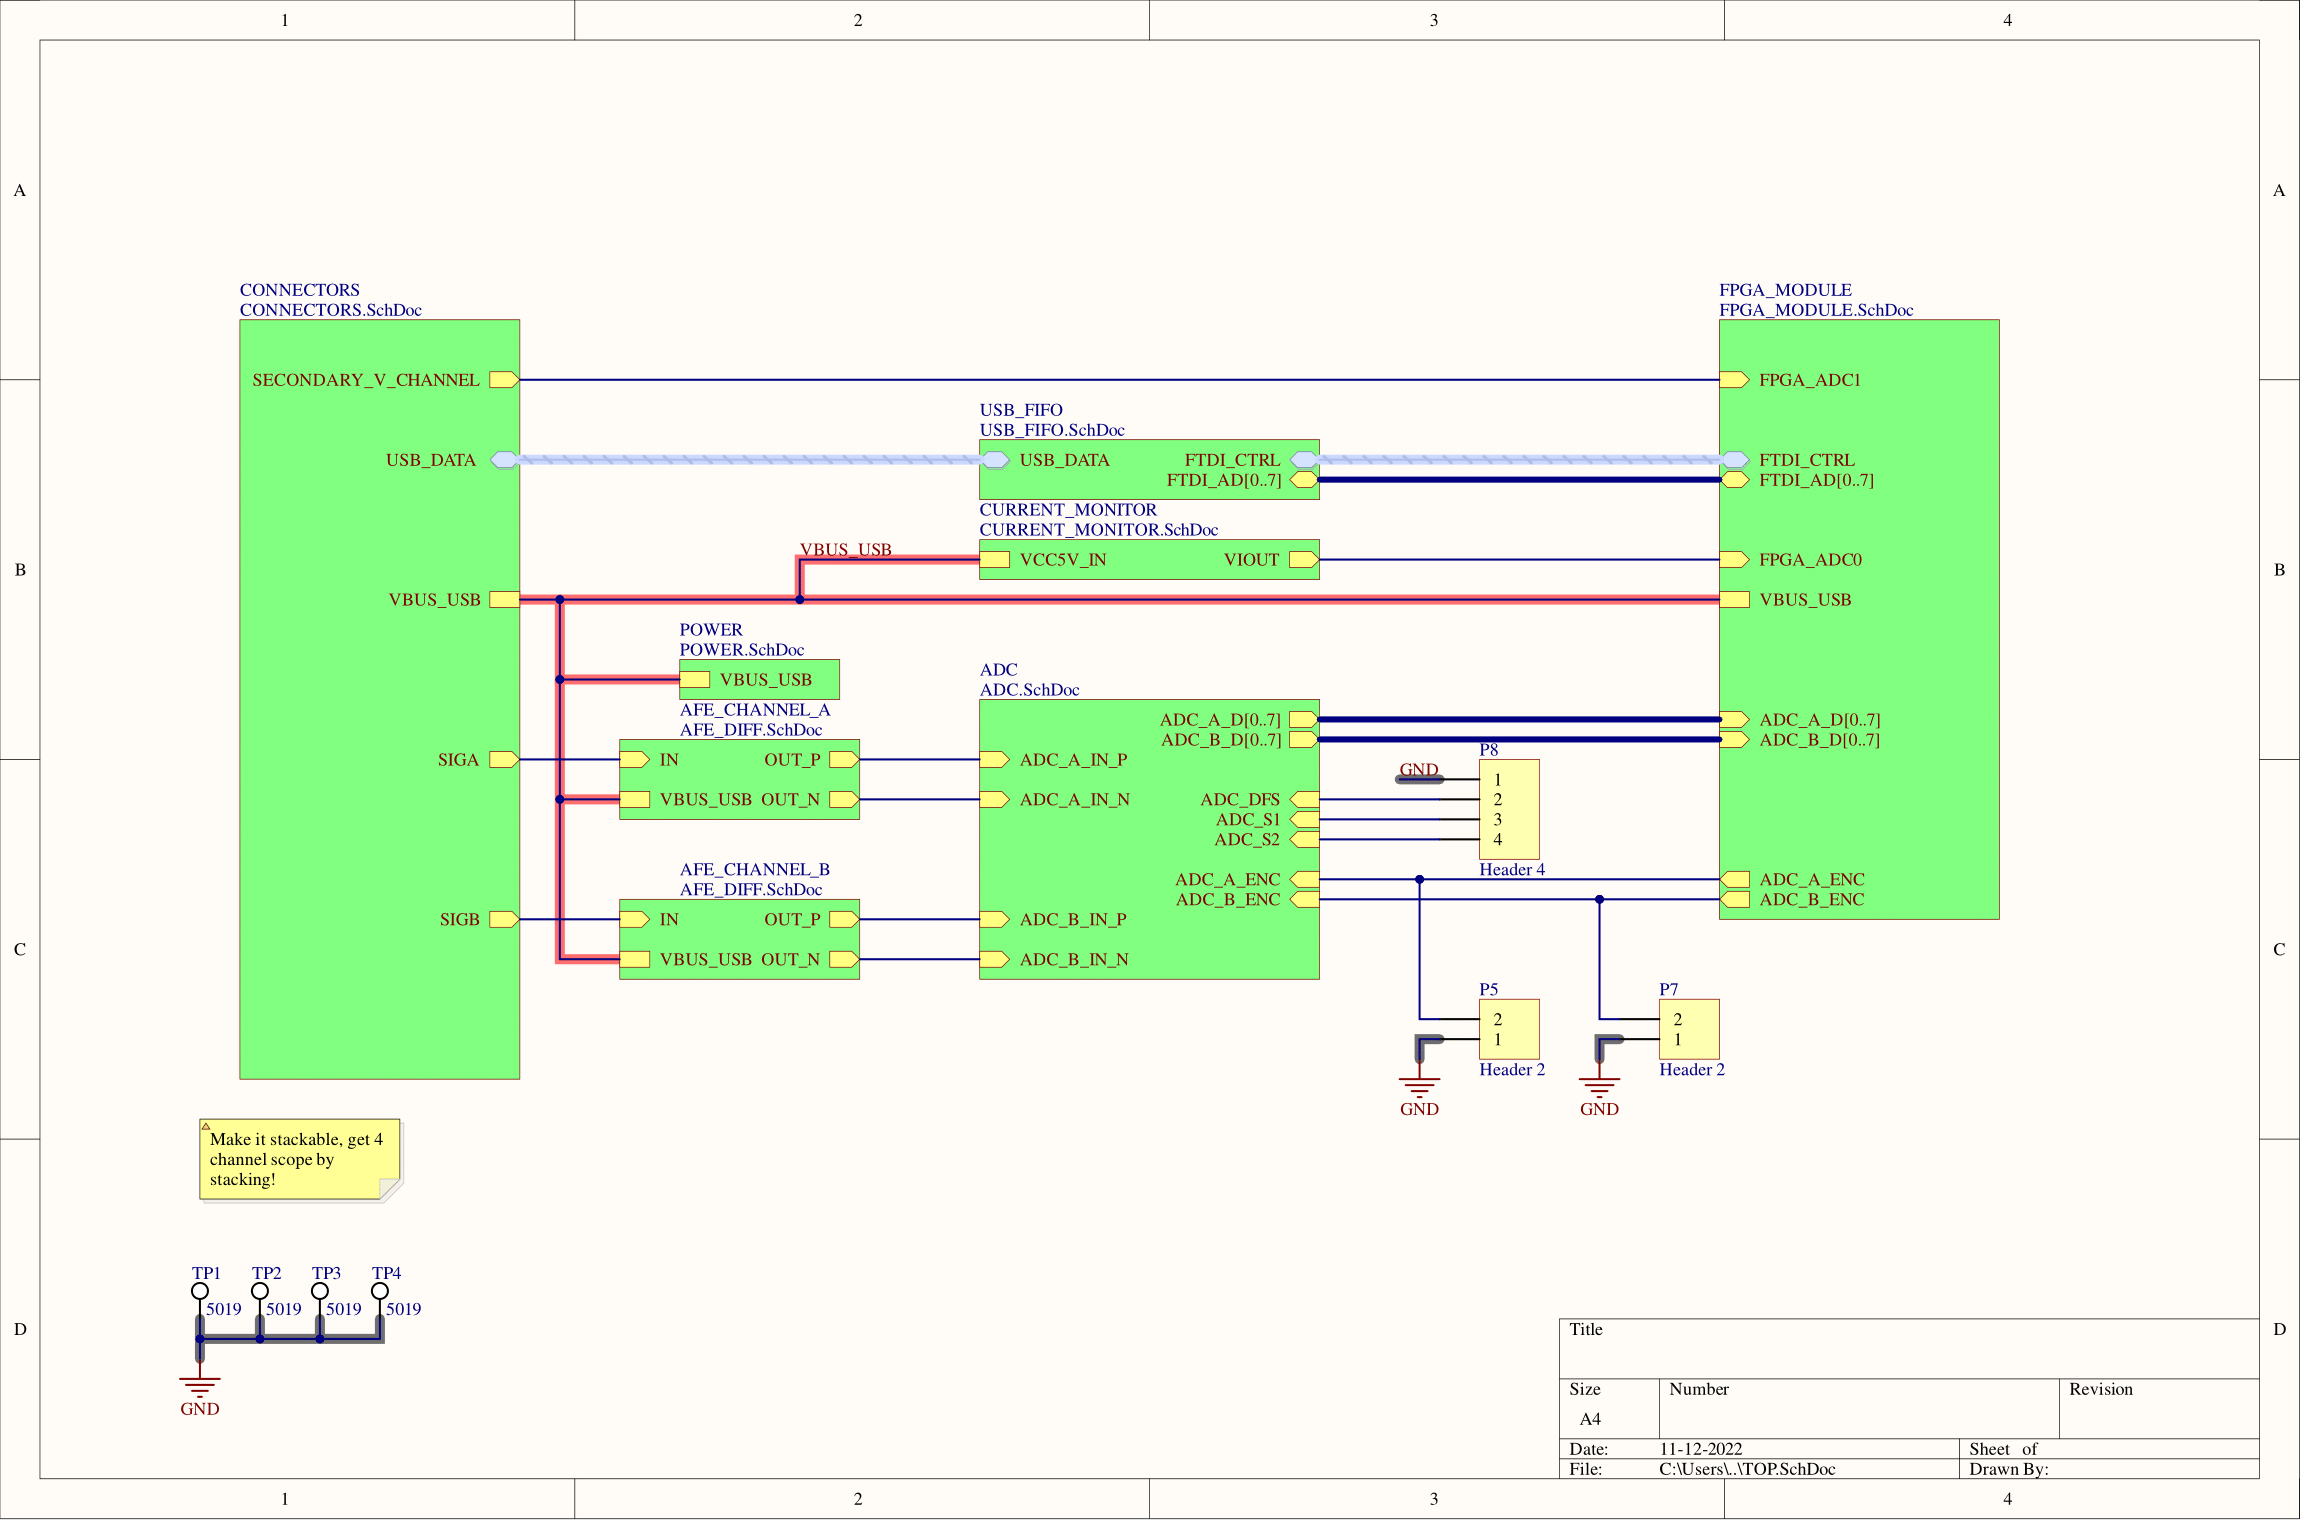
\includegraphics[height=15cm]{schematics/schematic1-1.png}
        \end{landscape}
    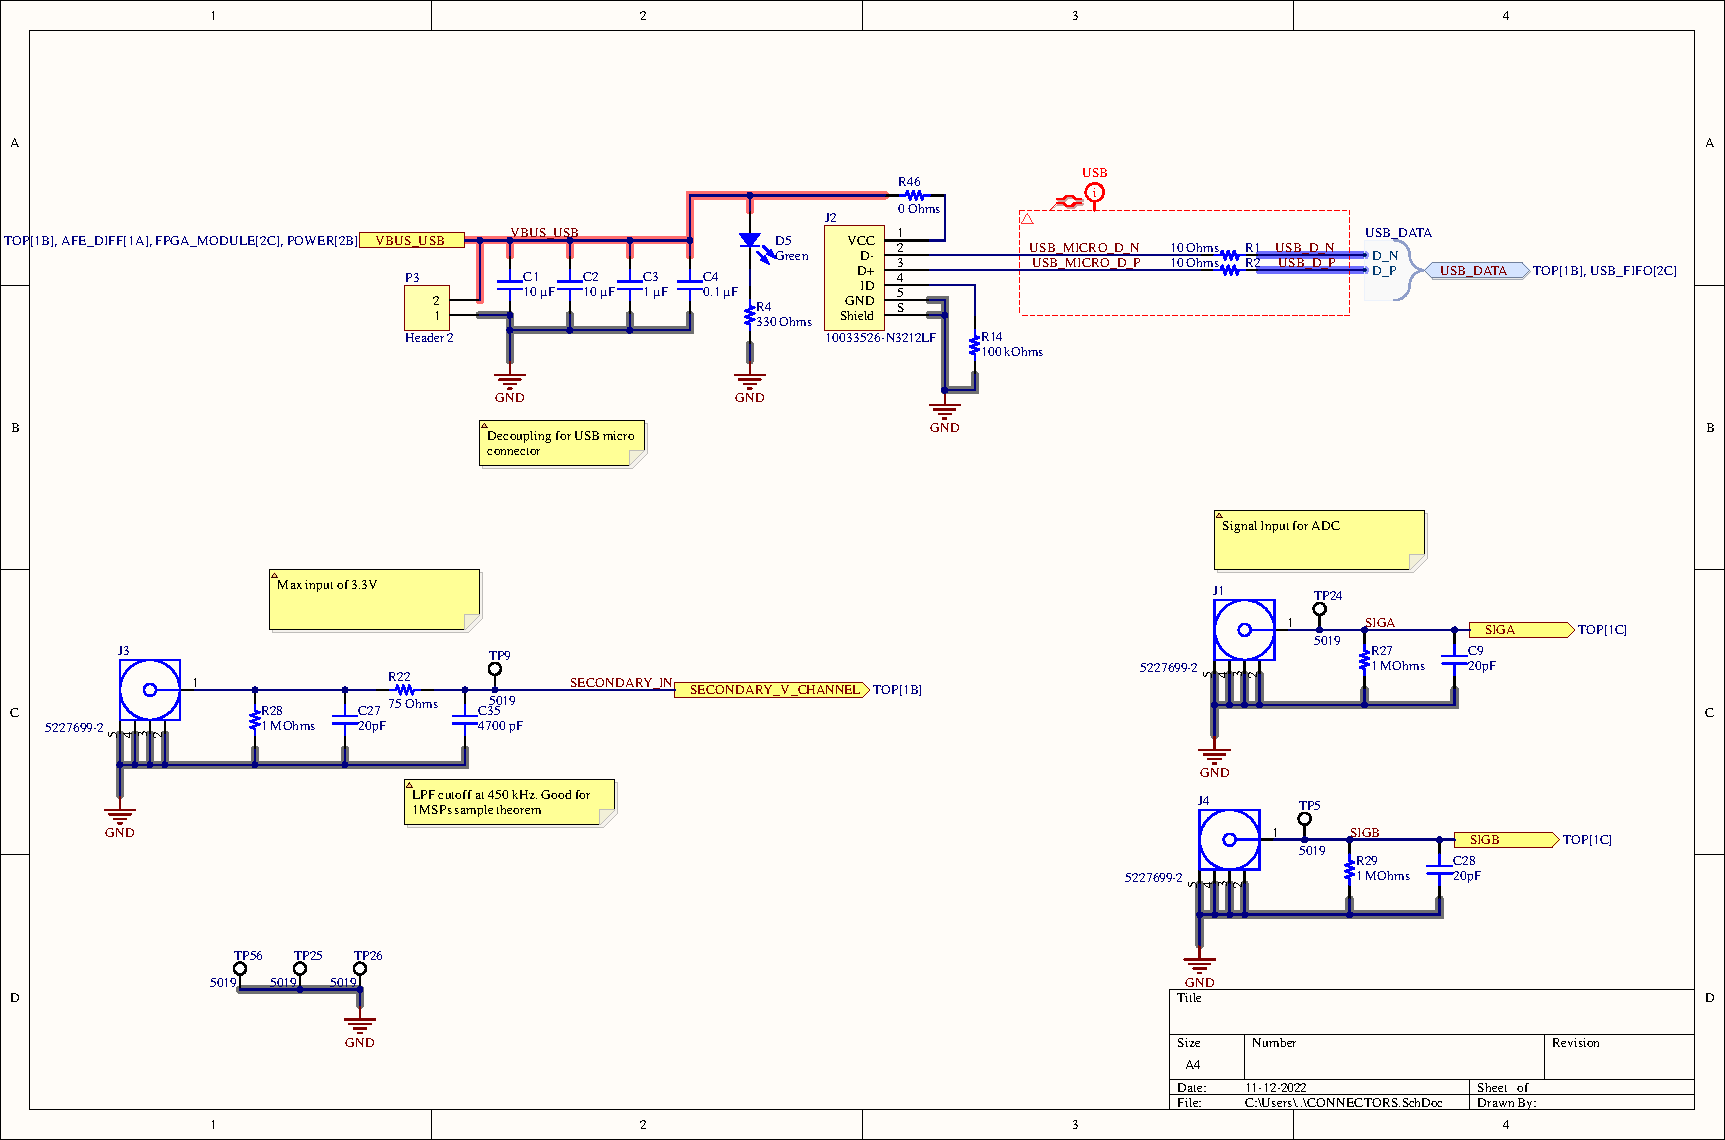
\includepdf[pages=-,landscape=true]{schematics/schematic2-8.pdf}

        \begin{landscape}
        \section{PCB Layout}
        \label{appendix:layout}
    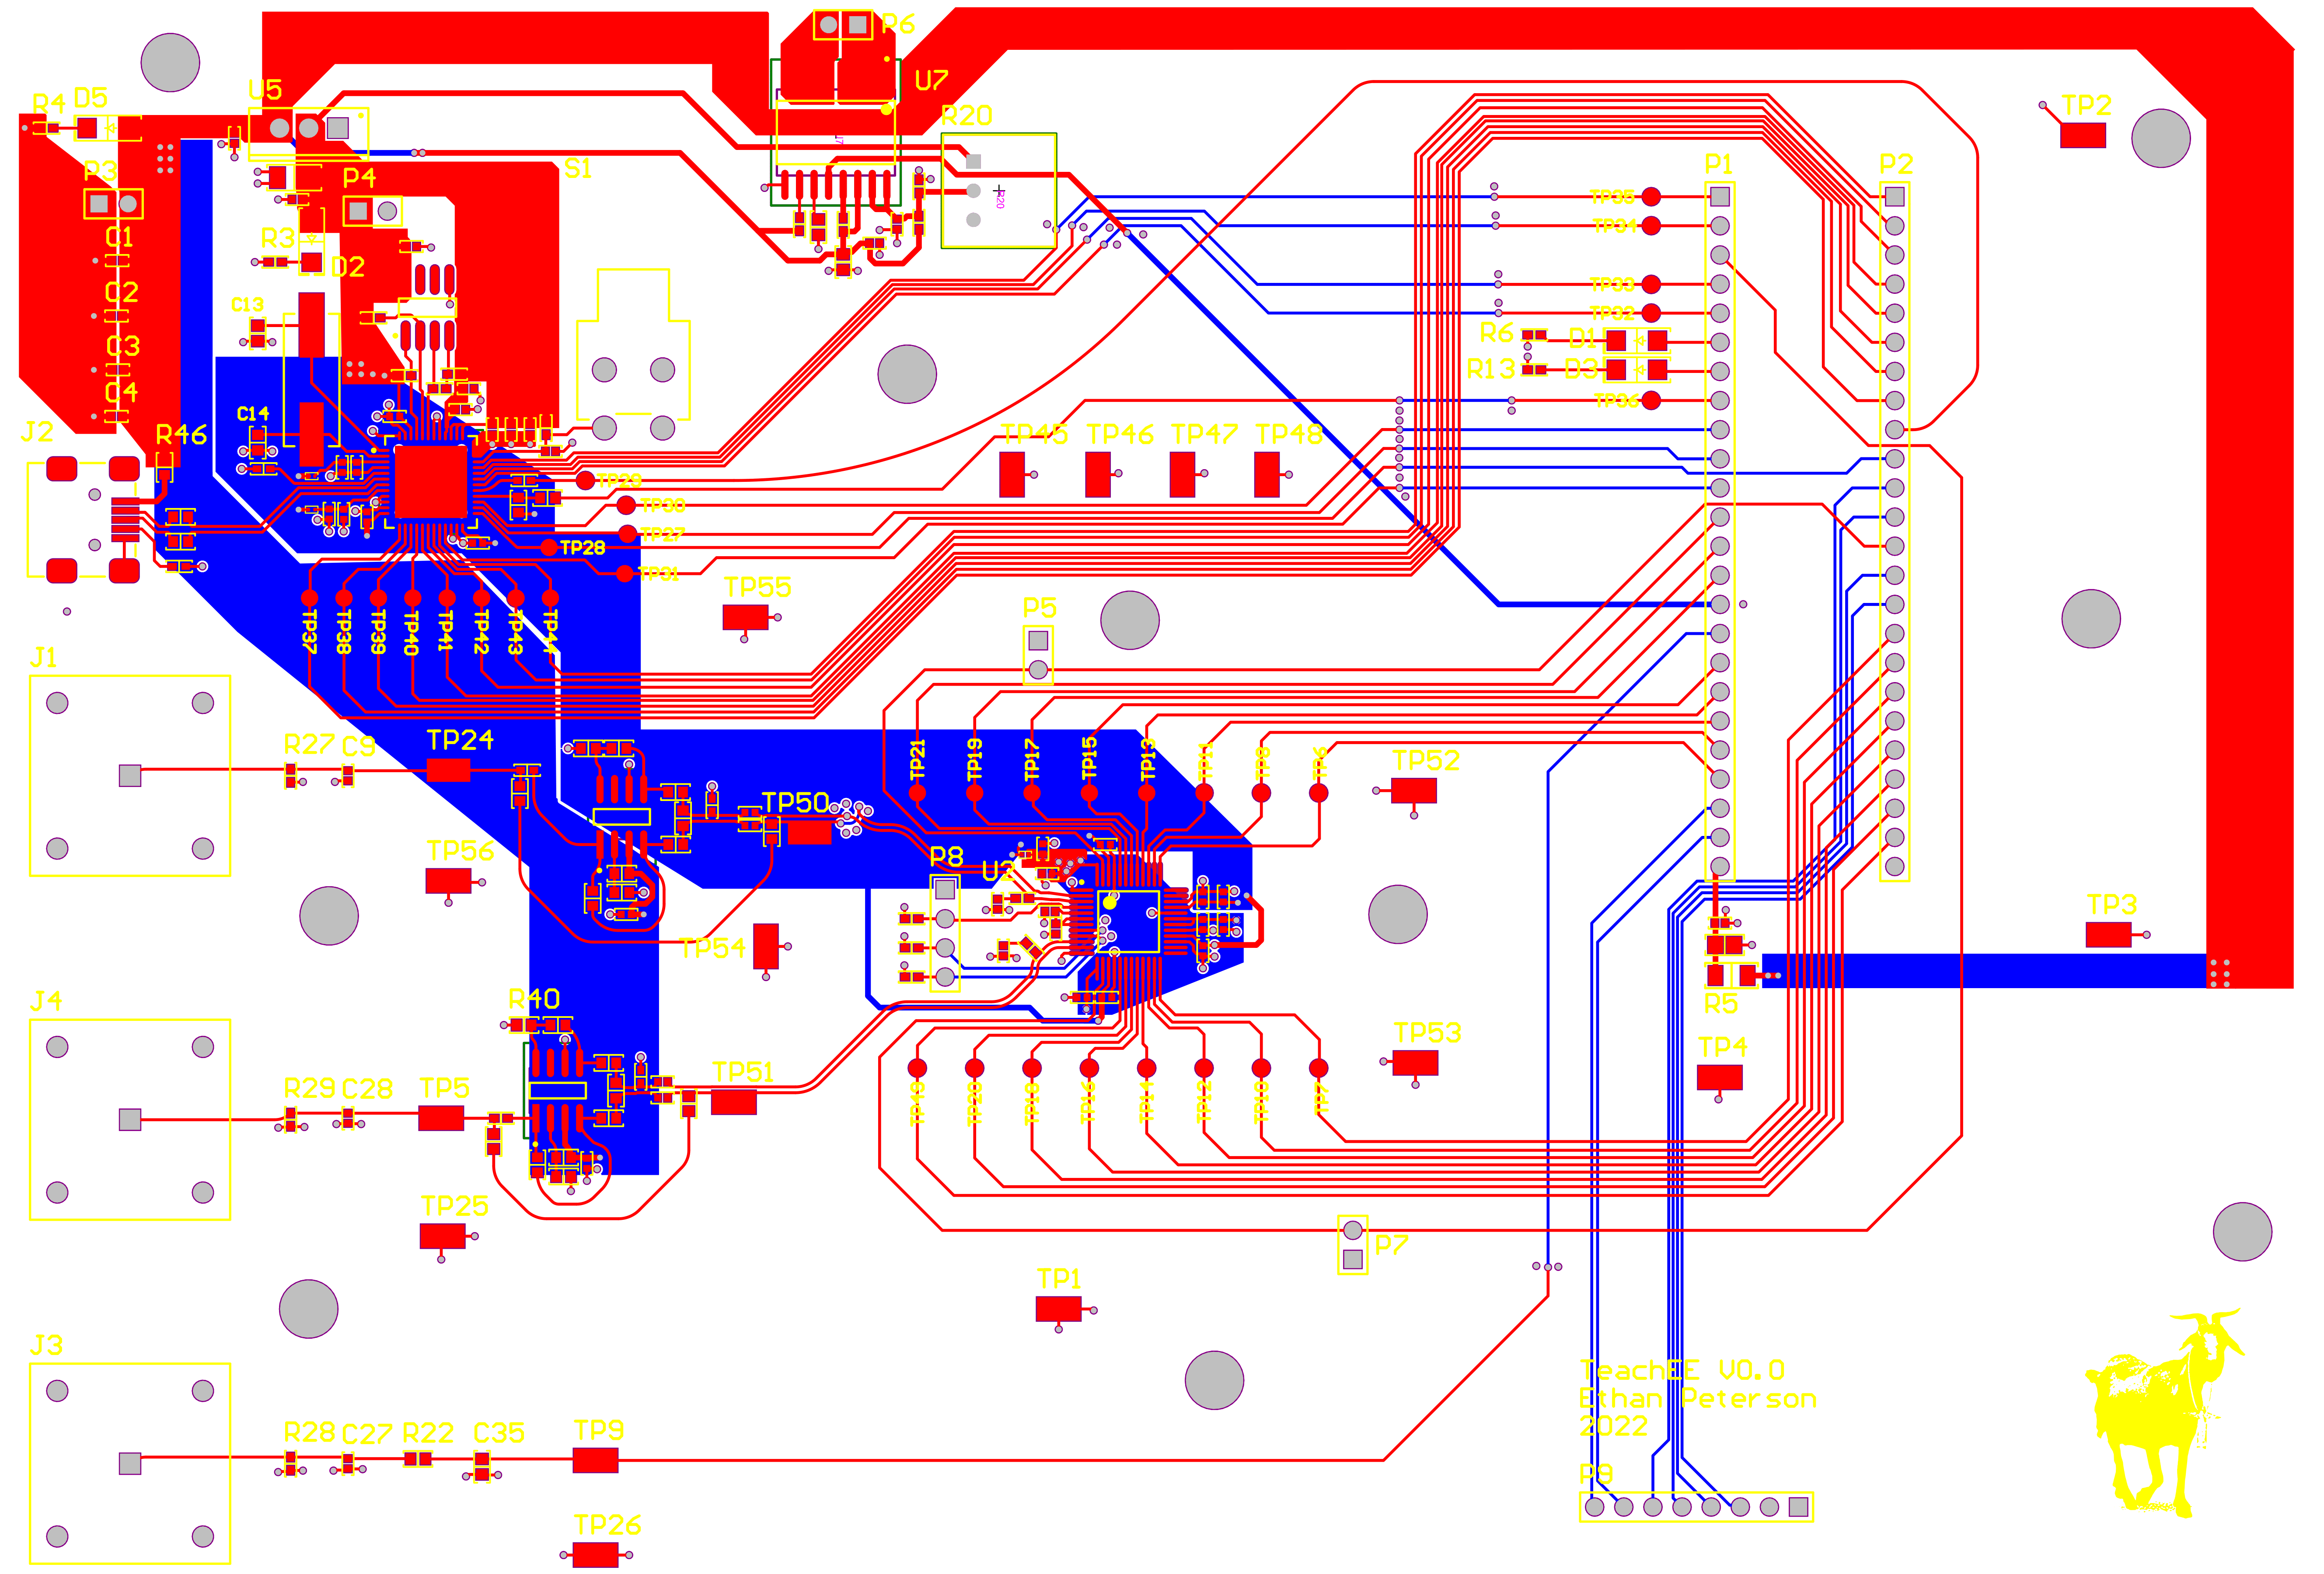
\includegraphics[height=15cm]{schematics/Layout.png}
        \end{landscape}

        \section{PCB Bill of Materials}
        \label{appendix:bom}
    \begin{table}[h!]
    \begin{tabular}{p{1.7in}|p{0.3in}|p{0.8in}|p{0.7in}|p{0.7in}|p{1in}}
        \textbf{Designator} & \textbf{QTY} & \textbf{Description} & \textbf{Comment} & \textbf{Footprint} & \textbf{Part Number} \\ \hline 
        C1, C2, C37, C48 & 4 & CAP CER 10UF 10V X5R 0402 & 10 µF & CAP 0402\_1005 & CL05A106MP8NUB8 \\ \hline
        C3 & 1 & CAP CER 1UF 10V X7S 0402 & 1 µF & CAP 0402\_1005 & GRM155C71A105KE11D \\ \hline
        C4, C11, C16, C17, C18, C19, C20, C21, C22, C24, C26, C29, C30, C38, C39, C40, C41, C42, C43, C44, C45, C46, C47, C50\_AFE\_CHANNEL\_A, C50\_AFE\_CHANNEL\_B, C52\_AFE\_CHANNEL\_A, C52\_AFE\_CHANNEL\_B, C53\_AFE\_CHANNEL\_A, C53\_AFE\_CHANNEL\_B & 29 & CAP CER 0.1UF 50V X5R 0402 & 0.1 µF & CAP 0402\_1005 & CGA2B3X5R1H104M050BB \\ \hline
        C5, C12, C32, C34 & 4 & CAP CER 0.1UF 10V X7R 0402 & 0.1µF & CAP 0402\_1005 & 0402ZC104KAT2A \\ \hline
        C6 & 1 & CAP CER 10UF 16V X5R 1206 & 10 µF & CAP 1206\_3216 - 0.8MM & EMK316BJ106MD-T \\ \hline
        C7 & 1 & CAP CER 10UF 35V X6S 0805 & 10 µF & CAP 0805\_2012 & GRM21BC8YA106KE11L \\ \hline
        C8, C15, C23, C25 & 4 & CAP CER 4.7UF 16V X5R 0402 & 4.7 µF & CAP 0402\_1005 & CL05A475MO5NUNC \\ \hline
        C9, C27, C28 & 3 & CAP CER 20PF 25V NP0 0402 & 20pF & CAP 0402\_1005 & 04023U200JAT2A \\ \hline
    \end{tabular}
    \end{table}

    \newpage

    \begin{table}[h!]
    \begin{tabular}{p{1.7in}|p{0.3in}|p{0.8in}|p{0.7in}|p{0.7in}|p{1in}}
        \textbf{Designator} & \textbf{QTY} & \textbf{Description} & \textbf{Comment} & \textbf{Footprint} & \textbf{Part Number} \\ \hline 
        C10 & 1 & CAP MLCC 0.01UF 100V X7R 0402 & 10000 pF & CAP 0402\_1005 & HMK105B7103KVHFE \\ \hline
        C13, C14 & 2 & CAP CER 36PF 100V NP0 0603 & 36pF & CAP 0603\_1608 & 06031A360JAT2A \\ \hline
        C31 & 1 & CAP CER 1UF 16V X7R 0603 & 1 µF & CAP 0603\_1608 & C0603C105K4RACAUTO \\ \hline
        C33, C35 & 2 & CAP CER 0603 4.7NF 16V X7R 10\% & 4700 pF & CAP 0603\_1608 & C0603C472K4RECAUTO \\ \hline
        C51\_AFE\_CHANNEL\_A, C51\_AFE\_CHANNEL\_B & 2 & CAP CER 15PF 25V C0G/NP0 0603 & 15 pF & CAP 0603\_1608 & C0603C150J3GACAUTO \\ \hline
        D1, D3 & 2 & LED SMD & Blue & LED 1206\_3216 BLUE & APTL3216QBC/D-01 \\ \hline
        D2, D5 & 2 & LED SMD & Green & LED 1206\_3216 GREEN & APTL3216ZGCK-01 \\ \hline
        FB1, FB2, FB3 & 3 & FERRITE BEAD 33 OHM 0201 1LN & 33 Ohms @ 100 MHz & FER 0201\_0603 & MMZ0603F330CT000 \\ \hline
        J1, J3, J4 & 3 & Jack BNC Connector, 1 Position, Height 16.26 mm, Tail Length 6.35 mm, -55 to 85 degC, RoHS, Tube & 5227699-2 & & 5227699-2 \\ \hline
        J2 & 1 & CONN RCPT MINI USB B 5POS SMD RA & & & 10033526-N3212LF \\ \hline
    \end{tabular}
    \end{table}
    \newpage
    \begin{table}[h!]
        \begin{tabular}{p{1.7in}|p{0.3in}|p{0.8in}|p{0.7in}|p{0.7in}|p{1in}}
        \textbf{Designator} & \textbf{QTY} & \textbf{Description} & \textbf{Comment} & \textbf{Footprint} & \textbf{Part Number} \\ \hline 
        R1, R2 & 2 & RES SMD 10 OHM 0.1\% 1/10W 0603 & 10 Ohms & RES 0603\_1608 & CRT0603-BY-10R0ELF \\ \hline
        R3, R6, R13 & 3 & RES 220 OHM 1\% 1/8W 0402 & 220 Ohms & RES 0402\_1005 & CRGP0402F220R \\ \hline
        R4 & 1 & RES SMD 330 OHM 5\% 1/16W 0402 & 330 Ohms & RES 0402\_1005 & AC0402JR-07330RL \\ \hline
        R5 & 1 & 1206 40 AMP JUMPER & 0 Ohms & RES 1206\_3216 & JR1206X40E \\ \hline
        R7 & 1 & RES SMD 12K OHM 0.1\% 1/16W 0402 & 12 kOhms & RES 0402\_1005 & CPF0402B12KE1 \\ \hline
        R8, R9, R10, R11, R17, R18, R19, R21, R32, R33, R34 & 11 & RES 10K OHM 0.1\% 1/10W 0402 & 10 kOhms & RES 0402\_1005 & RP73PF1E10KBTD \\ \hline
        R12 & 1 & RES 1.8K OHM 1\% 1/16W 0402 & 1.8 kOhms & RES 0402\_1005 & RC0402FR-071K8L \\ \hline
        R14 & 1 & RES SMD 100K OHM 0.1\% 1/16W 0402 & 100 kOhms & RES 0402\_1005 & CPF0402B100KE \\ \hline
        R15, R46 & 2 & RES SMD 0 OHM JUMPER 1/2W 0603 & 0 Ohms & RES 0603\_1608 & 5110 \\ \hline
        R22 & 1 & RES SMD 75 OHM 1\% 1/10W 0603 & 75 Ohms & RES 0603\_1608 & AC0603FR-0775RL \\ \hline
        R26 & 1 & RES 24 OHM 1\% 1/16W 0402 & 24 Ohms & RES 0402\_1005 & RC0402FR-0724RL \\ \hline
        \end{tabular}
    \end{table}
    \newpage
    \begin{table}[h!]
        \begin{tabular}{p{1.7in}|p{0.3in}|p{0.8in}|p{0.7in}|p{0.7in}|p{1in}}
        \textbf{Designator} & \textbf{QTY} & \textbf{Description} & \textbf{Comment} & \textbf{Footprint} & \textbf{Part Number} \\ \hline 
        R27, R28, R29 & 3 & RES 1M OHM 1\% 1/16W 0402 & 1 MOhms & RES 0402\_1005 & RMCF0402FT1M00 \\ \hline
        R36\_AFE\_CHANNEL\_A, R36\_AFE\_CHANNEL\_B & 2 & RES SMD 523 OHM 0.1\% 1/16W 0402 & 523 Ohms & RES 0402\_1005 & ERA-2ARB5230X \\ \hline
        R37\_AFE\_CHANNEL\_A, R37\_AFE\_CHANNEL\_B, R40\_AFE\_CHANNEL\_A, R40\_AFE\_CHANNEL\_B, R41\_AFE\_CHANNEL\_A, R41\_AFE\_CHANNEL\_B & 6 & RES SMD 500 OHM 0.05\% 1/10W 0603 & 500 Ohms & RES 0603\_1608 & TNPU0603500RAZEN00 \\ \hline
        R39\_AFE\_CHANNEL\_A, R39\_AFE\_CHANNEL\_B, R43\_AFE\_CHANNEL\_A, R43\_AFE\_CHANNEL\_B & 4 & RES 50 OHM 5\% 1/8W 0603 & 50 Ohms & RES 0603\_1608 & CH0603-50RJNTA \\ \hline
        R42\_AFE\_CHANNEL\_A, R42\_AFE\_CHANNEL\_B & 2 & RES SMD 4.02K OHM 1\% 1/10W 0603 & 4.02 kOhms & RES 0603\_1608 & AC0603FR-074K02L \\ \hline
        R44\_AFE\_CHANNEL\_A, R44\_AFE\_CHANNEL\_B & 2 & RES SMD 1K OHM 1\% 1/10W 0603 & 1 kOhms & RES 0603\_1608 & AA0603FR-071KL \\ \hline
        R45\_AFE\_CHANNEL\_A, R45\_AFE\_CHANNEL\_B & 2 & RES 25 OHM 0.1\% 1/20W 0402 & 25 Ohms & RES 0402\_1005 & FC0402E25R0BST0 \\ \hline
        S1 & 1 & SWITCH PUSH SPST-NO 0.4VA 28V & &  & AB11AH-HA \\ \hline
        TP1, TP2, TP3, TP4, TP5, TP9, TP24, TP25, TP26, TP45, TP46, TP47, TP48, TP50, TP51, TP52, TP53, TP54, TP55, TP56 & 20 & Test Point, 1 Position SMD, RoHS, Tape and Reel & 5019 & KSTN5019 & 5019 \\ \hline
        U1 & 1 & IC HS USB TO UART/FIFO 48QFN & FT232 & QFN-48 & FT232HQ-REEL \\ \hline
        \end{tabular}
    \end{table}
    \newpage
    \begin{table}[h!]
        \begin{tabular}{p{1.7in}|p{0.3in}|p{0.8in}|p{0.7in}|p{0.7in}|p{1in}}
        \textbf{Designator} & \textbf{QTY} & \textbf{Description} & \textbf{Comment} & \textbf{Footprint} & \textbf{Part Number} \\ \hline 
        U2 & 1 & Dual 8-Bit AD Converter with Parallel Interface, 40MSPS, -40 to +85 degC, ST-48, Pb-Free, Tray &  & ST-48M & AD9288BSTZ-40 \\ \hline
        U3\_AFE\_CHANNEL\_A, U3\_AFE\_CHANNEL\_B & 2 & IC ADC DRIVER 8SOIC & AD8138 & R-8-IPC\_A & AD8138ARZ-R7 \\ \hline
        U5 & 1 & Fixed Low Drop Positive Voltage Regulator, 3.3V, 3-Pin TO-220 & LD1117 & TO220 & LD1117V33C \\ \hline
        U6 & 1 & 2K, 128x16-bit, 2.5V Microwire Serial EEPROM, 8-Pin SOIC 150mil, Commercial Temperature, Tape and Reel & 93LC56 & SOIC8 & 93LC56BT/SN \\ \hline
        U7 & 1 & CURRENT SENSOR & ACS720 &  & ACS720KLATR-15AB-T \\ \hline
        Y1 & 1 & CRYSTAL 12.0000MHZ 20PF SMD & 12 MHz & ABLS & ABLS-12.000MHZ-20-B-3-H-T \\ \hline
        \end{tabular}
    \end{table}
    \end{appendices}
\end{document}
